% gabs's template

\documentclass[12pt]{article}

% Packages
\usepackage{amsmath} % For mathematical symbols and equations
\usepackage{amssymb} % For additional mathematical symbols
\usepackage{amsthm} % For theorem environments
\usepackage{geometry} % For page margins
\usepackage{fancyhdr} % For custom headers and footers
\usepackage{enumitem} % For custom lists
\usepackage{tikz} % For drawing lines
\usepackage{titlesec} % For section formatting
\usepackage{graphicx} % For including graphics
\usepackage{caption} % For caption formatting
\usepackage[most]{tcolorbox} % For colored boxes
\usepackage{xcolor} % For color definitions

% Page Layout
\geometry{a4paper, margin=1in}

% Define custom colors using hexadecimal values
\definecolor{rose}{HTML}{d18a8a} % Hex color for rose
\definecolor{foam}{HTML}{8da4b4} % Hex color for foam
\definecolor{gold}{HTML}{ea9d34} % Hex color for gold
\definecolor{iris}{HTML}{c4a7e7} % Hex color for iris
\definecolor{love}{HTML}{e5687a} % Hex color for love

% Theorem Definitions
\newtheorem{theorem}{Theorem}[section]
\newtheorem{lemma}[theorem]{Lemma}
\newtheorem{corollary}[theorem]{Corollary}
\newtheorem{definition}[theorem]{Definition}
\newtheorem{example}[theorem]{Example}

% Header and Footer
\pagestyle{fancy}
\fancyhf{}
\fancyhead[L]{Course Name}
\fancyhead[C]{Report Title}
\fancyhead[R]{\today}
\fancyfoot[C]{\thepage}

% Formatting
\titleformat{\section}{\normalfont\Large\bfseries}{\thesection}{1em}{}
\titleformat{\subsection}{\normalfont\large\bfseries}{\thesubsection}{1em}{}
\titleformat{\subsubsection}[runin]{\normalfont\normalsize\bfseries}{\thesubsubsection}{1em}{}

% Define tcolorbox styles with updated colors
\tcolorboxenvironment{problem}{colback=rose!10!white,colframe=rose!80!black,
fonttitle=\bfseries, title=Problem}
\tcolorboxenvironment{answer}{colback=foam!10!white,colframe=foam!80!black,
fonttitle=\bfseries, title=Answer}
\tcolorboxenvironment{proof}{colback=iris!10!white,colframe=iris!80!black,
fonttitle=\bfseries, title=Proof}
\tcolorboxenvironment{drawing}{colback=gold!10!white,colframe=gold!80!black,
fonttitle=\bfseries, title=Drawing}
\tcolorboxenvironment{example}{colback=love!10!white,colframe=love!80!black,
fonttitle=\bfseries, title=Example}

\title{Solutions to Problem Set}
\author{Your Name}
\date{\today}

\begin{document}

\maketitle

\section{Introduction}
Brief introduction about the problem set and methodology.

\section{Problem 1}
\begin{problem}
State the question here.
\end{problem}

\begin{answer}
Provide the answer here. Use \texttt{amsmath} for complex equations and \texttt{amssymb} for symbols. For example $x^2+x^3$:

\begin{equation}
    x^2+x^3 = x_3
\end{equation}

\end{answer}

\begin{proof}
Provide the proof here. Use \texttt{amsthm} for theorem environments if needed.
\end{proof}


\begin{drawing}
If needed, include a drawing or diagram. For example:
\begin{figure}[h!]
    \centering
    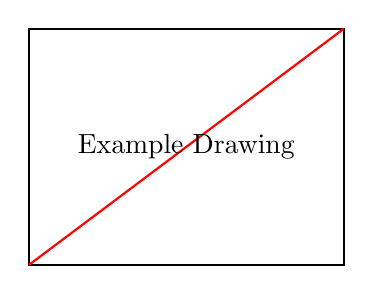
\begin{tikzpicture}
        % Example drawing
        \draw[thick] (0,0) rectangle (4,3);
        \draw[thick, red] (0,0) -- (4,3);
        \node at (2,1.5) {Example Drawing};
    \end{tikzpicture}
    \caption{A sample drawing.}
    \label{fig:example-drawing}
\end{figure}
\end{drawing}

\begin{example}
Provide any relevant examples or additional explanations.
\end{example}

\section{Problem 2}
\begin{problem}
State the question here.
\end{problem}

\begin{answer}
Provide the answer here.
\end{answer}

\begin{proof}
Provide the proof here.
\end{proof}

\begin{drawing}
Include any necessary diagrams or illustrations.
\end{drawing}

\begin{example}
\[
\sum_{k}^{n} seila
.\] 
Provide examples or additional explanations if applicable.
\end{example}

% Add more problems as needed

\section{Conclusion}
Summarize the findings or conclusions of the report.

\end{document}
